% !TEX root = DesignDocument.tex


\chapter{User Documentation}

\section{Overall Guide}
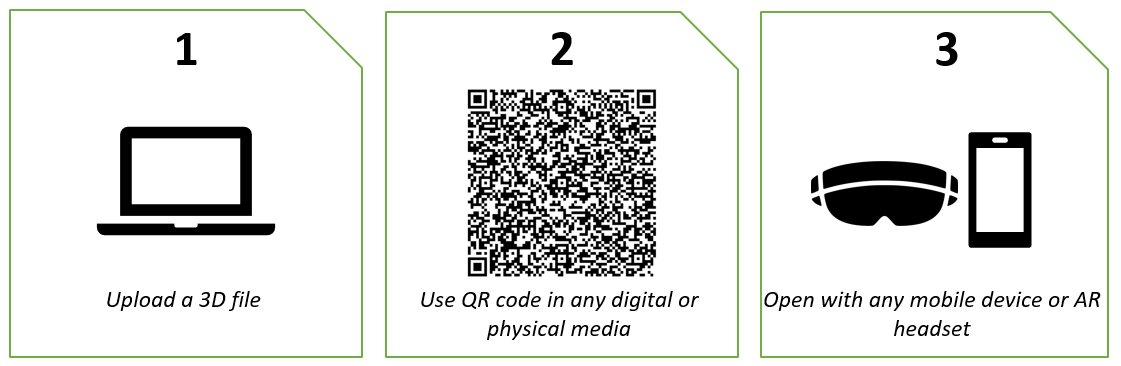
\includegraphics[width=\textwidth]{AugmentedEducationHowTo.png}

\section{User Guide for Website}
\begin{itemize}
    \item Public Content: displays all publicly viewable files.
    \begin{itemize}
        \item Displayed files may be searched or filtered using the Search and Filter bar at the top of the listing.
        \item Clicking a file will reveal options for selecting a file type in which to downloaded the file or for which to a have a linked QR code generated.
        \item QR codes must be generated for mobile devices and all non-mobile devices separately. 
    \end{itemize}
    \item My Content: displays a user's public and private files.
    \begin{itemize}
        \item User's private and public files are displayed in separate tables.  
        \item Tables may be searched or filtered using the Search and Filter bar at the top of the listings.
        \item Clicking a file will reveal options for selecting a file type in which to downloaded the file or for which to a have a linked QR code generated.
        \item QR codes must be generated for mobile devices and all non-mobile devices separately. 
        \item Clicking a file will reveal an options for deleting a file from the cloud. Any QR codes previously associated with the file will no longer work. 
    \end{itemize}
    \item Upload: allows a user to upload a file.
    \begin{enumerate}
        \item Add a file to be uploaded.  
        \item Optionally add a material file to be uploaded. 
        \item Optionally add an alternate display name for the file.
        \item Optionally add a description for the file.
        \item Select whether the file will be public or private.
        \item Press "Upload."
        \item A notification message will appear to indicate success or failure of the upload. 
    \end{enumerate}
    \item Help: displays platform guide for users. 
\end{itemize}

\section{User Guide for HoloLens}

\section{User Guide for Mobile App}

\section{Demos}

See Appendix \ref{ch:support} for demonstrations of the platform in use. 

\section{User Guide for Capturing Demos}

\subsection{Website}
\begin{itemize}
    \item For screenshots:
    \begin{enumerate}
        \item Navigate to the desired page. 
        \item Find and open Snipping Tool, a default application on windows. 
        \item Select "New" and then select the capture area. 
        \item Save or right-click to copy screenshot. 
    \end{enumerate}
    \item For videos:
    \begin{enumerate}
        \item Open Microsoft PowerPoint.
        \item Navigate to the "Insert" tab. 
        \item Select "Screen Recording." 
        \item Select the recording area.
        \item Press "Record."
        \item To end recording, press the Window's logo key, shift, and "Q" all together.
        \item The recording will now appear in your PowerPoint. 
        \item To save the recording to your desktop, right-click it and select "Save media as..."
    \end{enumerate}
\end{itemize}

\subsection{HoloLens}
\begin{enumerate}
    \item With the HoloLens on, verbally say "Cortana, record this," to begin recording.
    \item Perform the "bloom" motion of opening a closed fist to finish recording.
	\item Recordings will be saved to the One Drive of the account signed in on the HoloLens. Access the One Drive to share and view recordings. 
\end{enumerate}

\subsection{Mobile App}
\begin{enumerate}
    \item Download any screen recording application. 
    \item Open the screen recording application and press the "record" icon.
    \item To finish recording, press the "record" icon again. 
    \item Select "Save."
    \item The video will be saved to the mobile device's gallery and may be shared.
\end{enumerate}

%This section should contain the basis for any end user documentation for the system. 
% End user documentation would cover the basic steps for setup and use of the system. 
% It is likely that the majority of this section would be present in its own document 
%to be delivered to the end user.  However, it is recommended the original is contained 
%and maintained in this document. 
%
%%\newpage   %% 
%%%  The user guide can be an external document which is included here if necessary ...
%%%  a single source is the way to go.
%
%\section{User Guide}
%
%The source for the user guide can go here.    You have some options for how to handle the user docs.  If you have some {\tt newpage} commands around the guide then you can just print out those pages.   If a different formatting is required, then have the source in a separate file {\tt userguide.tex} and include that file here.  That file can also be included into a driver (like the senior design template) which has the client specified formatting.  Again, this is a single source approach.   
%
%
%%% \newpage  %%  if needed ...
%\section{Installation Guide}
%
%
%%% \newpage  %%  if needed ...
%\section{Programmer Manual}
%
